
\subsection*{From RGB LEDs to VGA}
\begin{itemize}
    \item \textbf{RGB LED:} Basic color representation with \( R, G, B \) channels.
    \item \textbf{VGA Protocol:} Standard for analog video output from computers.
\end{itemize}

\subsection*{Communicating with VGA Protocol}

The VGA protocol is implemented using various pins on a connector. It supports several analog signals for color and synchronization. Here's a simplified overview:

\begin{minipage}[t]{0.5\textwidth}
    \textbf{Pinout Diagram:}
    \begin{center}
        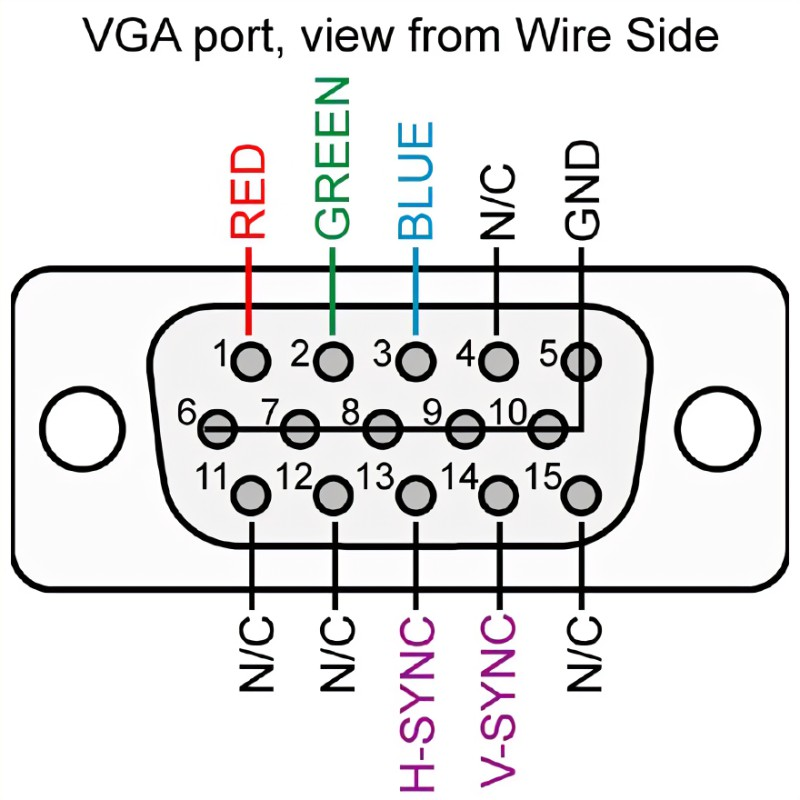
\includegraphics[width=\linewidth]{vga}
    \end{center}
\end{minipage}%
\begin{minipage}[t]{0.5\textwidth}
    \textbf{Signal Overview:}
    \begin{itemize}
        \item \textbf{Red, Green, Blue (RGB):} Analog signals for color intensity.
        \item \textbf{Horizontal Sync (HSYNC):} Synchronizes horizontal lines.
        \item \textbf{Vertical Sync (VSYNC):} Synchronizes vertical frames.
        \item \textbf{Analog Grounds:} Reference points for signals.
    \end{itemize}
\end{minipage}


\subsection*{Algorithm for Displaying an Image using VGA}

To display an image using the VGA protocol, the following steps are typically involved:

\begin{enumerate}
    \item \textbf{Initialize VGA Controller:} Set up registers for resolution, color depth, and synchronization timings.
    
    \item \textbf{Generate Horizontal Sync Signal (HSYNC):} Send pulses to synchronize the start of each line.
    
    \item \textbf{Generate Vertical Sync Signal (VSYNC):} Send pulses to synchronize the start of each frame.
    
    \item \textbf{Output RGB Signals:} For each pixel in the image:
    \begin{itemize}
        \item Calculate appropriate RGB voltages based on the color information of the pixel.
        \item Output analog signals through the corresponding RGB pins.
    \end{itemize}
    
    \item \textbf{Repeat for Each Frame:} Continuously update the screen by repeating the above steps for each frame.
\end{enumerate}


\pagebreak  

\subsection*{OpenGL: Revolutionizing Graphics Rendering}

% \noindent
% \begin{minipage}[t]{0.6\textwidth}
% The development of OpenGL (Open Graphics Library) transformed computer graphics by providing a standardized, cross-platform API for rendering 2D and 3D graphics. Initially developed by Silicon Graphics Inc. (SGI), OpenGL adopted a streamlined pipeline architecture for processing graphical data. The pipeline includes stages for vertex processing, primitive assembly, rasterization, and fragment processing. Each stage optimizes rendering tasks, leveraging hardware acceleration to achieve real-time visual output. OpenGL's versatility and efficiency have made it a cornerstone for interactive applications, ranging from video games to scientific simulations.
% \end{minipage}%
% \begin{minipage}[t]{0.25 \textwidth}
%     \vspace{2pt} % Ensure baseline alignment
%     % \centering
%     \begin{center}
%       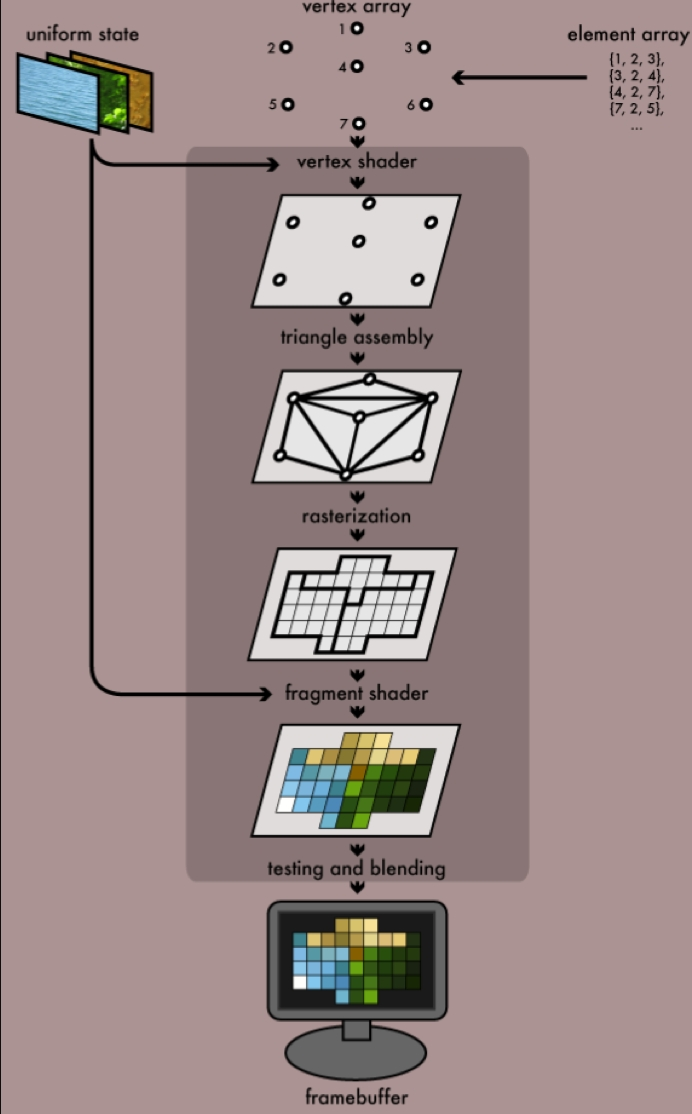
\includegraphics[width=\linewidth]{opengl_pipeline}
%     \end{center}
% \end{minipage}






% \subsection*{Hardware Acceleration and GPU Evolution}
% As demands for graphical complexity grew, dedicated Graphics Processing Units (GPUs) emerged to offload intensive rendering tasks from the CPU. GPUs specialize in parallel processing and include dedicated memory and computational units optimized for graphics operations. This shift enabled real-time rendering of complex scenes with dynamic lighting, textures, and effects. Modern GPUs continue to advance, incorporating technologies like ray tracing and tensor cores for enhanced realism and machine learning applications.

